\documentclass[11pt, letterpaper]{article}
\usepackage[utf8]{inputenc}

\usepackage[margin=1.25in]{geometry}

\usepackage{amsmath,amsfonts,amssymb,amsthm,pgf,tikz,enumerate,xcolor,graphicx,microtype}
\usepackage[colorlinks]{hyperref}

\usepackage{color}
\newcommand{\taylor}[1]{{\color{blue} \sf $\spadesuit\spadesuit\spadesuit$ Taylor: [#1]}}
%\newcommand{\collab}[1]{{\color{red} \sf $\spadesuit\spadesuit\spadesuit$ collab1: [#1]}}  %Dear Collaborator, make a macro for yourself here. 
\newcommand{\todo}[1]{{\color{purple} \sf $\spadesuit\spadesuit\spadesuit$ TODO: [#1]}}

\begin{document} 

\begin{center}
{\Large \sc Dupuy -- Math 1077  --Problem Bank\\ (with course objectives)}\\
last updated: \today
\end{center}

This file contains the Problem Bank and course objectives for Dupuy's Math 1077 course. 
All the problems for our quizzes are either going to be in this file or very similar to problems in this file.
\\

\vspace{1em} 

\noindent {\bf WARNING:} The problems in sections marked as ``unstable'' are subject to change.
The order and the titles of the sections might even change. 
Problems need to be tested and sometimes this takes a couple iterations. 

\vspace{1 em}

\noindent {\bf TEXTBOOKS:} The problems use the letters \emph{GH} and \emph{T} to indicate where problems are taken from.
\begin{itemize}
	\item \emph{GH}: \emph{The Magic Of Numbers} by Gross and Harris. (Available on the course webpage.)
	\item \emph{T}: \emph{Excursions in Modern Mathematics} by Tannenbaum.
\end{itemize}

\tableofcontents

\newpage

\section{Counting}
This material is ``officially'' covered in section 16.2 of Tannenbaum. 
A slower paced introduction is provided in Chapters 1-5 of \emph{The Magic Of Numbers} by Gross and Harris (GH).

\subsection{Understanding Logarithms}
This was talked about in class.
\begin{enumerate}
	\item What is the approximate value of the logartihm of $12345689123456789$ in base 10?\footnote{No calculators for this one, there is a super cheap-o way of doing this.}
\end{enumerate}

\subsection{Understanding How To Count Numbers Between Numbers}
This is chapter 1 of GH. 
\begin{enumerate}
	\item How many numbers are there between 1776 and 2023? How many are even? How many are odd?  
\end{enumerate} 
\subsection{Understanding Permutations and the Multiplication Principle}
See GH Ch2 for this. 
\begin{enumerate}
	\item Suppose I have a textbook with a subsection of 5 problems that I want to rearrange for the next edition. How many ways can I do this for the next edition?
	\item Consider the make your own sandwich option at Mill Market in South Burlington: \begin{center}
		\url{https://themillmarket.com/deli-menu}
	\end{center}
    They have 9 proteins, 13 breads, 14 sauces, 6 cheeses, and 15 veggies. 
    Supposing you only use one sauce, one protein, one bread, one cheese, and any combination of veggies, how many sandwiches do they offer (you don't need to multiply out your answer)?
    If we do get crazy and allow any combination of cheeses, sauces, and proteins, how many sandwiches do they offer? How does this compare to the number of seconds the universe has existed?\footnote{Do not attempt to multiply out this number.}\footnote{The universe has existed for approximately $4.4\times 10^{17}$ seconds.}
\end{enumerate}
\subsection{Understanding the Subtraction Principle}
See GH Ch3 for this section.
\begin{enumerate}
	\item How many four digit PIN numbers are there with a repeat number?
	\item How many three digit numbers are there in base 10? [there are at least three ways of doing this]
	\item A license plate is three letters followed by a number between 100 and 999. How many license plates can you make following this rule? 
	\item A new style Massachusetts license plate as two letters A-Z and four numbers 0-9. How many new style Massachusetts license plates are there? How many are there if we require no repeat number and no repeat letter?
\end{enumerate}

\subsection{Understanding Collections}
This is GH Ch4. 
\begin{enumerate}
	\item How many ways are there to choose 2 objects from a subset of 10 objects?
	\item In basketball, only 5 people can be on the court at the same time. 
	If there is a team with 12 people on it, how many lineups can they make?
	\item Baskin Robbins has 31 flavors of ice cream. How many different three scoop ice cream servings are there? 
	\item How many ways are there to rearrange the letters in the word MISSISSIPPI? 
	\item T: 16.28
\end{enumerate}
\newpage

\section{Voting} 
A general reference for this material is Chapter 1 of Tannenbaum.
Note that the terminology that Tannenbaum uses slightly different terminology from class. 

\subsection{Understanding Burlington's 2009 Mayoral Race }

\noindent Problems 2--5 concern Table 1-31 of the book.
\begin{enumerate}
	\item Why is the Burlington 2009 Mayoral Election such an important example?
	\item (Most Votes Wins) T: 1.11
	\item (Borda Method) T:1.21
	\item (Instant Runoff) T:1.31
	\item (Round Robin) T:1.41
\end{enumerate}

\subsection{Understanding Slime Molds}
\begin{enumerate}
	\item What does the slime mold experiment have to do with ranked choice voting?
\end{enumerate}

\subsection{Understanding that Elections Are Fundamentally Flawed}
\begin{enumerate}
	\item What does the Arrow's Impossibility Theorem say?
	\item (Borda Violates Pairwise Comparison) T:1.51 [this example is telling us the Borda method is not cool]
	\item Come up with a simple example of a ranked choice election with three candidates where the Border, Instant-Runoff, and Pairwise comparison are all give different election results.
\end{enumerate}
\newpage


\section{Sets}

Here is a basic reference for set notation. 
Sets are just collections of things and there are a couple symbols we may use that help us count and talk about things.
Here is a basic reference: 
\begin{center}
	\url{https://www.mathsisfun.com/sets/sets-introduction.html}
\end{center}
We also use the following basic notation throughout this course:
\begin{align*}
\mathbb{N} &= \lbrace 1, 2, 3, \cdots \rbrace = \mbox{ (natural numbers) }\\
\mathbb{Z} &= \lbrace \ldots, -2,-1,0,1,2,\ldots,\rbrace = \mbox{(integers)}\\
\mathbb{Q} &= \lbrace \frac{p}{q} \colon p,q \in \mathbb{Z}, q\neq 0 \rbrace =\mbox{ (rational numbers)}\\
\mathbb{R} &= (\mbox{all numbers on the real number line})
\end{align*}
The way $\mathbb{Q}$ is defined is an example of ``set builder notation''.

\subsection{Understanding Union, Intersection, Subsets, Elements, Membership, and Cardinality}
\noindent For the following problems let $A= \lbrace a,b, c, 2\rbrace$ and $B = \lbrace a, 2, \pi\rbrace$ where $a,b$ and $c$ are abstract letters.  
\begin{enumerate}
	\item Write out $A \cap B$ as a set. What is the cardinality of $A\cap B$?
	\item Write out $A \cup B$ as a set. What is the cardinality of $A\cup B$?
	\item Write out $A\times B$ as a set. What the cardinality of $A\times B$?
	\item Write out $A\setminus B$ as a set. What is the cardinality of $A\setminus B$?
	\item Write out all of the subsets of $A$.
	\item Is it the case that $2 \in A$?
	\item Is it the case that $\pi \in A$?
	\item Is it the case that $\lbrace a,b \rbrace \subset A$?
\end{enumerate}

\subsection{Understanding Set Builder Notation}
\begin{enumerate}
	\item Write out the set of even numbers in set builder notation.
\end{enumerate}

\newpage

\section{Probability }
Here we follow Ch 16 of Tannenbaum. 
For additional help the reader should consult GH chapters Ch 4 and 5. 

\subsection{Understanding Sample Spaces}

\begin{enumerate}
	\item What does the sample space for a single coin flip look like?
	What does the sample space for two coin slips look like?
	What does the sample space for three coin flips look like?  (see Tannenbaum examples 16.1 and 16.2).
	\item Suppose you flip a coin 10 times. Which of the following sequences is more likely to occur?
	\begin{enumerate}
		\item $THHTHHTTHT$
		\item $TTTTTTTTTH$
	\end{enumerate}
	\item Suppose you flip a coin 10 times. Which of the following outcomes is more likely to occur? (see T: 17.74 for a similar problem)
	\begin{enumerate}
		\item Flipping 5 heads and 5 tails.
		\item Flipping 2 heads and 8 tails.
	\end{enumerate}
\end{enumerate}
\subsection{Understanding How to Compute Basic Probabilities}
\begin{enumerate}
	\item Suppose you are dealt two cards from a standard 52 card deck. 
	\begin{enumerate}
		\item What is the probability that the two cards are sequential (this includes $10J, JQ,QK,KA,A2$)?
		\item What is the probability that the two cards have the same suit?
		\item What is the probability that the two cards are a pair?
	\end{enumerate}
	\item You meet two people randomly on the street. What is the probability that they share the same birthday?
\end{enumerate}
	
\subsection{Understanding Expected Values}
\begin{enumerate}
	\item T:16.59
	\item T:16.57
	\item T:15.67
\end{enumerate}
\subsection{Understanding What to Do With Expected Values}
\begin{enumerate}
	\item Suppose you are in a poker hand and there is \$75 in the pot and your are put into a situation where you need to pay \$25 more to enter. 
	What does the probability that you have a winning hand need to be in order for this to be a good bet?	
\end{enumerate}

\subsection{Understanding $p$-Values}
\begin{enumerate}
	\item What is a $p$-value and how is one computed? (give an executive summary of the process without worrying about technical details).
	\item Explain the following xkcd cartoons related to $p$-values.
	\begin{enumerate}
		\item \url{https://xkcd.com/1478/}
		\item \url{https://xkcd.com/2533/}
		\item \url{https://xkcd.com/882/}
	\end{enumerate}
	\item 
	The following is from \emph{Currents of Fear} on Frontline.\footnote{I found this on \url{https://www.fallacyfiles.org/multcomp.html}}
	\begin{quote}
		…[I]n 1992, a landmark study appeared from Sweden. A huge investigation, it enrolled everyone living within 300 meters of Sweden's high-voltage transmission line system over a 25-year period. They went far beyond all previous studies in their efforts to measure magnetic fields, calculating the fields that the children were exposed to at the time of their cancer diagnosis and before. This study reported an apparently clear association between magnetic field exposure and childhood leukemia, with a risk ratio for the most highly exposed of nearly 4.
		
		…Surely, here was the proof that power lines were dangerous, the proof that even the physicists and biological naysayers would have to accept. But three years after the study was published, the Swedish research no longer looks so unassailable. 
		
		…[T]he original contractor's report…reveals the remarkable thoroughness of the Swedish team. Unlike the published article, which just summarizes part of the data, the report shows everything they did in great detail, all the things they measured and all the comparisons they made. …[N]early 800 risk ratios are in the report….1
	\end{quote}
	To be clear, the Swedish team took 800 thinks like leukemia and looked for associations between leukemia and living near power lines. 
	Why is it not surprising that one of these came up?
	With a $p$ value threshold of $0.05$, on average, how many ``risk ratios'' would we need to be computed to expect ``find some link''?
	\item In Ellenberg's \emph{How Not To Be Wrong} he proves that scientists are regularly abusing $p$-values. How does he do this? (You just need to say what goes into this roughly)
\end{enumerate}

\subsection{Understanding Coinflipping and the Central Limit Theorem}
\begin{enumerate}
	\item What is the plinko game? 
	\item What does coinflipping a coin 10 times in a row have to do with a single ball going through plinko with 10 levels? Why are these things similar? (draw a picture)
	\item If I flip 100 coins, how far away from a 50/50 split are we expected to be? (how many extra heads or tails are expected on average?)
	\item Your friend Taylor loves to flip coins and owns a fair coin he flips all the time. 
	\begin{enumerate}
		\item After an amazing 15 streak of heads, he is insists that the next flip will more likely be tails in order to make up for the number of heads that just occured. What mistakes is he making?
		\item After flipping 100 coins what is the expected disparity between the number of heads and number of tails?
	\end{enumerate}
\end{enumerate}

\newpage

\section{Graphs and Networks}
 
\subsection{Understanding the Basic Terminology of Graphs and Networks}
\begin{enumerate}
	\item T:5.3, 5.4
	\item T: 5.7
\end{enumerate}

\subsection{Understanding what the Koenigsberg Bridges Problem}
The material for this section is 5.1 and 5.2 of Tannenbaum in \emph{The Mathematics of Getting Around}. 

We started this section with the \emph{Koenigsberg Bridges Puzzle}. 
A map of the city of Koenigsberg is pictured in Figure~\ref{F:seven-bridges}.
\begin{figure}[h]
	\begin{center}
		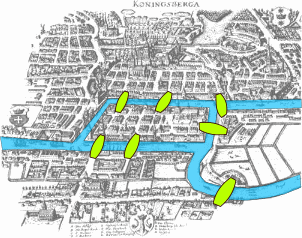
\includegraphics[scale=0.5]{konigsberg_bridges.png}
	\end{center}
	\caption{The city of Koenigsburg and its seven bridges.}\label{F:seven-bridges}
\end{figure}
The \emph{Koenigsberg Bridges Puzzle} asks the following: is there a way to take a walk in the city where you cross each bridge exactly once?

\begin{enumerate}
	\item (Turn a city map into a graph) T:5.20.
	\item Consider the city in the previous problem. Can we walk across all of the bridges exactly once without repeating? Why or why not?
	\item (Which graphs have Euler Circuits) 5.32
	\item Consider the appartment with a floor plan pictured in Figure~\ref{F:floor-plan}.
	Explain why it is impossible to make a tour of the appartment using all of the doors exactly once. 
	
	\footnote{This puzzle was given to a collaborator of mine in 5th grade as an extra credit problem. 
	It is impossible. 
	}
	
	\begin{figure}[h]
		\begin{center}
			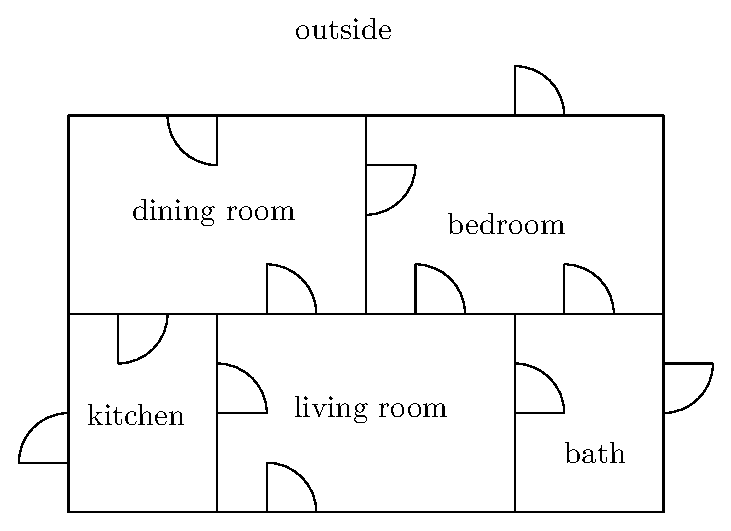
\includegraphics[scale=0.5]{floor-plan}
		\end{center}
		\caption{The floor plan of a ground floor appartment, its rooms, and the various doors connecting each of the rooms.  }\label{F:floor-plan}
	\end{figure}
	
	
	
	
\end{enumerate}

\subsection{Understanding the Traveling Salesman Problem}

\begin{enumerate}
	\item Why is the Traveling Salesman Problem so hard?
	\item (Find Hamiltonian Paths) 6.2
	\item (Count the TSP Paths) 6.55 \footnote{I will not quiz on this since it is longer.}
	\item (Ore's Condition) 6.68 and 6.69 \footnote{I will not quiz on this problem since it is harder}
\end{enumerate}

\subsection{Understanding the Three Houses Three Utilities Problem}
This section is about planar graphs which isn't covered in the book, so here is a great video lecture series on the topic:
\begin{center}
	\href{https://www.youtube.com/playlist?list=PLGxuz-nmYlQPgIHbqWtgD-F7NnJuqs4fH}{Sarada Herke's Lectures on Planar Graphs}
\end{center}

I motivated the section with the \emph{Three Houses Three Utilities} puzzle.
The \emph{Three Houses and Three Utilities} puzzle says that there are three houses that need to be connected to three utilities but none of the lines are allowed to cross. How do you configure your lines so that each of the houses can have all three ultilities? The initial setup for the \emph{Three Houses and Three Utilities} puzzle is pictured in Figure~\ref{F:three-houses}.
\begin{figure}[h]
	\begin{center}
		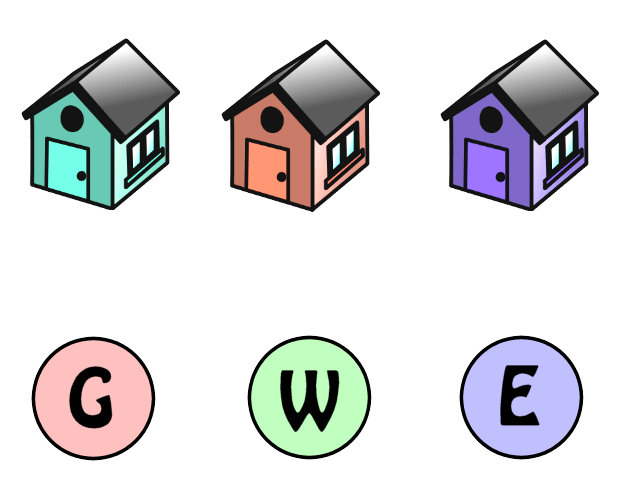
\includegraphics[scale=0.25]{three-houses.png}
	\end{center}
	\caption{A image of the three houses and three utilities problem.  Image taken from \href{http://puzzles.nigelcoldwell.co.uk/twentysix.htm}{Nigel Coldwell's webpage.} }\label{F:three-houses}.
\end{figure}
The following questions are about explaining why the \emph{Three Houses and Three Utilities} puzzle is impossible. 

\begin{enumerate}
	\item What is a planar graph?
	\item Draw a graph and a minor of the graph. 
	\item Draw $K_{3,3}$ and $K_5$.
	\item Give an example of a planar graph.
	\item Give an example of a non-planar graph that is not $K_{3,3}$ or $K_5$.
	\item Consider the graph pictured in Figure~\ref{F:non-planar}. Can this graph be made planar or not? Why? (Hint: contract $de$, $hf$, and $fg$.)
	\item Why is the \emph{Three Houses Three Utilities} puzzle impossible? \footnote{My 5th grade Mathematics teacher gave this problem to us as students as extra credit.}
\end{enumerate}

	
\begin{figure}[h]
	\begin{center}
		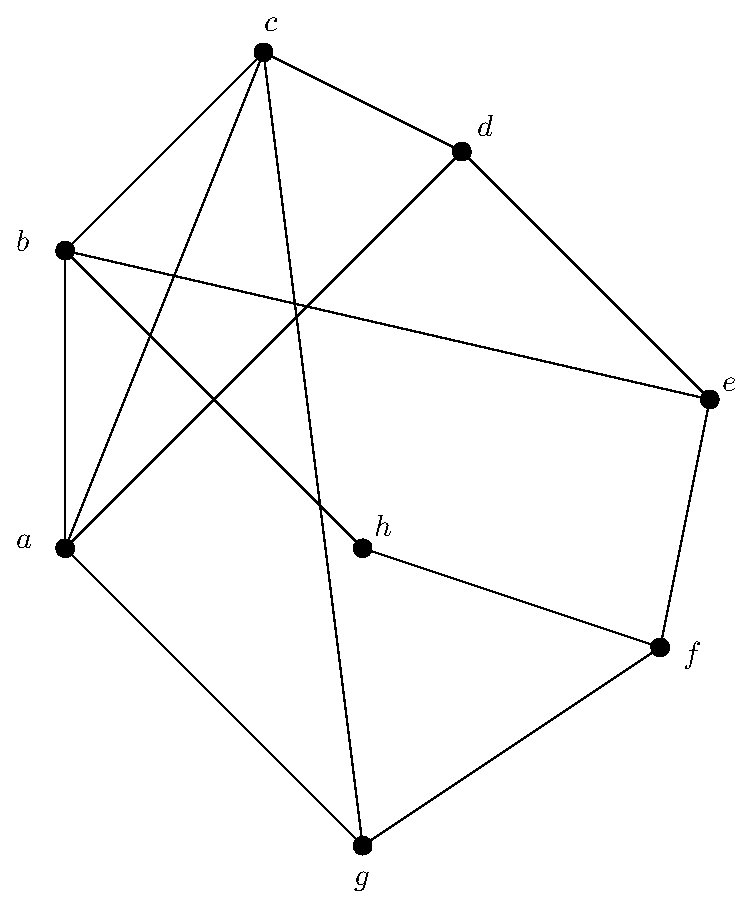
\includegraphics[scale=0.25]{non-planar.eps}
	\end{center}
	\caption{A graph for a homework problem. }\label{F:non-planar}.
\end{figure}

\newpage

\section{Symmetry and the Golden Ratio (unstable)}

\subsection{Prisoner Problem}
\begin{enumerate}
	\item Write consider the permutation $f: \lbrace 1,2,3,4\rbrace \to \lbrace 1,2,3,4\rbrace$ given by 
	 $$ 1 \mapsto 3,  \quad 2 \mapsto 4, \quad 3 \mapsto 1, \quad 4\mapsto 2.$$
	Write this in permutation notation.
	\item Why does the prisoner problem work?
\end{enumerate}

\subsection{Dihedral Groups}
\begin{enumerate}
	\item 
\end{enumerate}

\newpage

\section{Statistics (unstable) }
The webpage \url{https://www.explainxkcd.com} may be helpful for some of the problems featuring xkcd cartoons.
\subsection{Understanding How To Read Graphs}

\begin{enumerate}
	\item Explain the following xkcd cartoons.
	\begin{enumerate}
		\item \url{https://xkcd.com/1007/}
		\item \url{https://xkcd.com/1945/}
	\end{enumerate}
\end{enumerate}

\subsection{Understanding How People Are Reckless With Extrapolation}
\begin{enumerate}
    \item Give one real life example of how people carelessly used linear regression or some other fitting technique to conclude something wrong and/or dangerous.
    \item Explain the following xkcd comics related to extrapolation.
    \begin{enumerate}
    	\item \url{https://xkcd.com/476/}
    	\item \url{https://xkcd.com/605/}
    \end{enumerate}
    \item In \emph{Life on the Mississippi} Mark Twain writes 
    \begin{quote}
    	The Mississippi between Cairo and New Orleans was twelve hundred and fifteen miles long one hundred and seventy-six years ago. It was eleven hundred and eighty after the cut-off of 1722. It was one thousand and forty after the American Bend cut-off. It has lost sixty-seven miles since. Consequently, its length is only nine hundred and seventy-three miles at present. Now, if I wanted to be one of those ponderous scientific people, and "let on" to prove what had occurred in the remote past by what had occurred in a given time in the recent past, or what will occur in the far future by what has occurred in late years, what an opportunity is here! … Please observe: In the space of one hundred and seventy-six years the Lower Mississippi has shortened itself two hundred and forty-two miles. That is an average of a trifle over one mile and a third per year. Therefore, any calm person, who is not blind or idiotic, can see that in the Old Oolitic Silurian Period, just a million years ago next November, the Lower Mississippi River was upward of one million three hundred thousand miles long, and stuck out over the Gulf of Mexico like a fishing-rod. And by the same token any person can see that seven hundred and forty-two years from now the Lower Mississippi will be only a mile and three-quarters long, and Cairo and New Orleans will have joined their streets together, and be plodding comfortably along under a single mayor and a mutual board of aldermen. There is something fascinating about science. One gets such wholesale returns of conjecture out of such a trifling investment of fact.
    \end{quote}
    I don't really have a good problem here. I just wanted you to know that even Mark Twain was making fun of this.
    \item What is the Laffer Curve? (what was the original example)
    \item Come up with an example of something that obeys the Laffer Curve rule.
\end{enumerate}


\subsection{Understanding How To Estimate The Number of German Tanks}
\begin{enumerate}
	\item What ideas went into the estimation of German Tanks by Statisticians in World War 2?
    \item (Capture Recapture Example) 14.61
\end{enumerate}

\subsection{Understanding Sample Sizes}
\begin{enumerate}
    \item 
    As of Monday, Jan 16, 2023: basketball-reference.com shows currently shows that your cousin, Trevor Hudgins, as the league leader in unqualified three-point percentage (3P\%): 
    \begin{center} \url{https://www.basketball-reference.com/leagues/NBA_2023_totals.html#totals_stats::fg3_pct}
    \end{center}
    Your family is very proud. How do you explain to explain to your grandma at Christmas that cousin Trevor is not as good as Steph Curry at three pointers? 
\end{enumerate}\footnote{
There is a common fallacy that because someone has disease $X$ and people from group $Y$ have disease 
}

\subsection{Understanding Base Rate Fallacies}
\begin{enumerate}
    \item Jersey girls are three times more likely to have a gel manicure (this is totally made up). Your friend sees a girl with a gel manicure and concludes that she must be from Jersey. What mistake is your friend making?
    
    \item Taylor and Gloria are close friends. Gloria shares the terrible news with Taylor  that her husband Albert has lung cancer. Knowing that the CDC says smokers are 15-30 more likely to get lung cancer than non-smokers Taylor suspects that Albert was probably a smoker. This is false and only about 65\% of lung cancer patients are not smokers.\footnote{https://www.lungevity.org/for-supporters-advocates/lung-cancer-awareness/lung-cancer-statistics} What mistake did Taylor make?
    \footnote{
    	There is a common fallacy that because someone has disease $X$ and people from group $Y$ have a higher incidence of disease $X$ that someone with disease $X$ is more likely to come from group $Y$. 
    	Humans want to make this mistake all the time. 
    	Try to think of a couple examples. 
    }
\end{enumerate}

\subsection{Understanding Correlation}
\begin{enumerate}
 \item Some people on the internet argue that men are smarter than women in the following way: they point out that brain size is correlated with IQ scores and that IQ scores are correlated with gender. What is wrong with this argument?
 \end{enumerate}
\newpage

\section{Decision Theory (unstable) }


\subsection{Understanding Utils}
\begin{enumerate}
	\item Why does \$100 dollars mean a lot less to a billionaire than to someone making minimum wage?
	\item 
\end{enumerate}
\newpage






\end{document}